\section{LO1: Visualization basics, chart types}

\subsection{Line Charts}

Line charts are often the first choice for illustrating temporal data (Figure \ref{fig:line_chart_good}). This is because they excel at showing trends over time, making them ideal for financial, scientific, and statistical data. The linear representation helps the audience quickly identify increases or decreases in values over a specified period. They are also useful for showing the relationship between two variables, such as the correlation between GDP and life expectancy.

\begin{figure}[h]
    \centering
    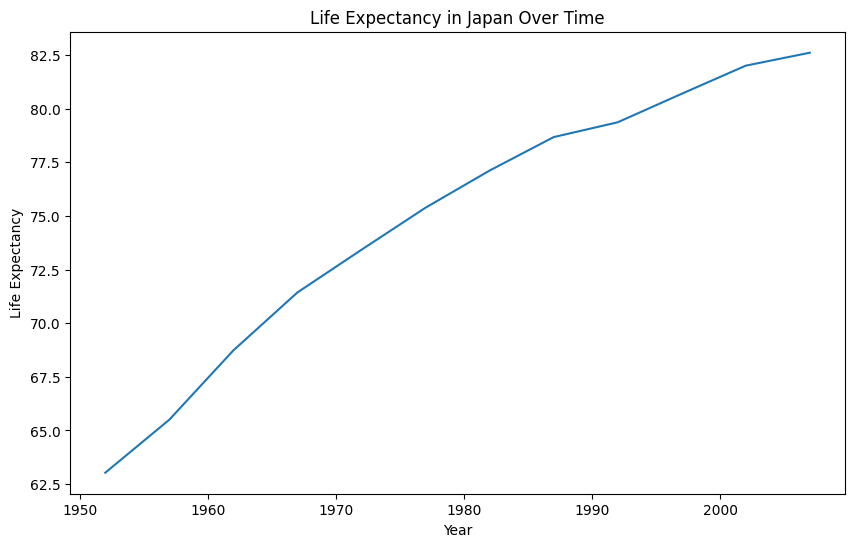
\includegraphics[width=0.5\textwidth]{images/plots/lo1_good_example_life_expectancy_japan.png} 
    \caption{Line Chart of the Life Expectancy in Japan Over Time}
    \label{fig:line_chart_good}
\end{figure}

However, line charts are less appropriate for comparing individual categories side-by-side. This is because lines imply a connection or progression between points, which may not be meaningful for unrelated categories \cite{fewNowYouSee2009}.

\subsection{Pie Charts}

Pie charts are one of the most commonly misused chart types (Figure \ref{fig:pie_chart_bad}). They are best used to represent proportional or percentage data, often for a total that amounts to 100\%. However, they can be misleading as the human eye struggles to accurately compare the area or angle of pie slices, especially as the number of categories increases \cite{tufteVisualDisplayQuantitative2015}.

\begin{figure}[h]
    \centering
    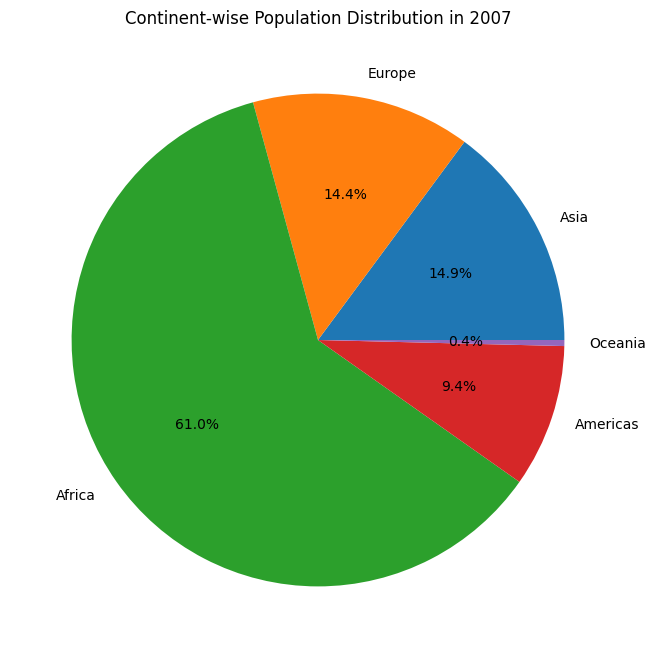
\includegraphics[width=0.5\textwidth]{images/plots/lo1_bad_example_population_distribution_2007.png} 
    \caption{Pie chart of Continent-wise Population Distribution in 2007}
    \label{fig:pie_chart_bad}
\end{figure}

\subsection{Bar Charts}

Bar charts are highly versatile and can be used in various applications (Figure \ref{fig:bar_chart_good}). The reason they are so effective for comparisons is that the length of bars allows for easy, accurate judgments of value differences. This makes them suitable for comparing data across a large number of different categories.

\begin{figure}[h]
    \centering
    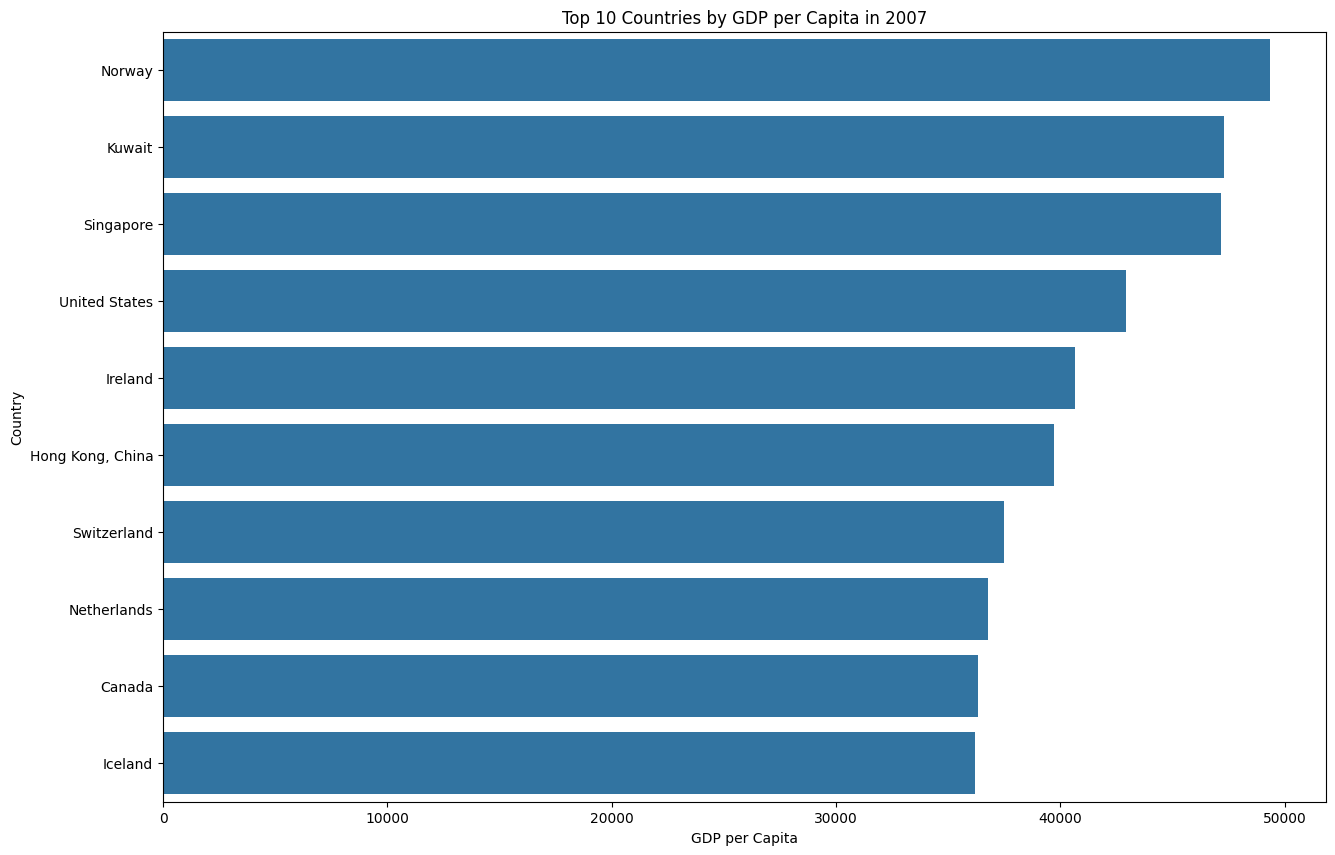
\includegraphics[width=0.5\textwidth]{images/plots/lo1_good_example_top10_gdp_2007.png} 
    \caption{Bar chart of the top 10 Countries by GDP per Capita in 2007}
    \label{fig:bar_chart_good}
\end{figure}

Bar charts are less suitable for showing trends over time, as they do not imply a temporal progression between categories \cite{heerTourVisualizationZoo2010}.

\subsection{Boxplots}

Boxplots are a powerful tool for understanding the distribution of data across different categories (Figure \ref{fig:boxplot_good}). They display a five-number summary of the data: the minimum, first quartile, median, third quartile, and maximum. This provides a robust summary of the data's central tendency, spread, and presence of outliers \cite{tukeyExploratoryDataAnalysis1977}.

\begin{figure}[h]
    \centering
    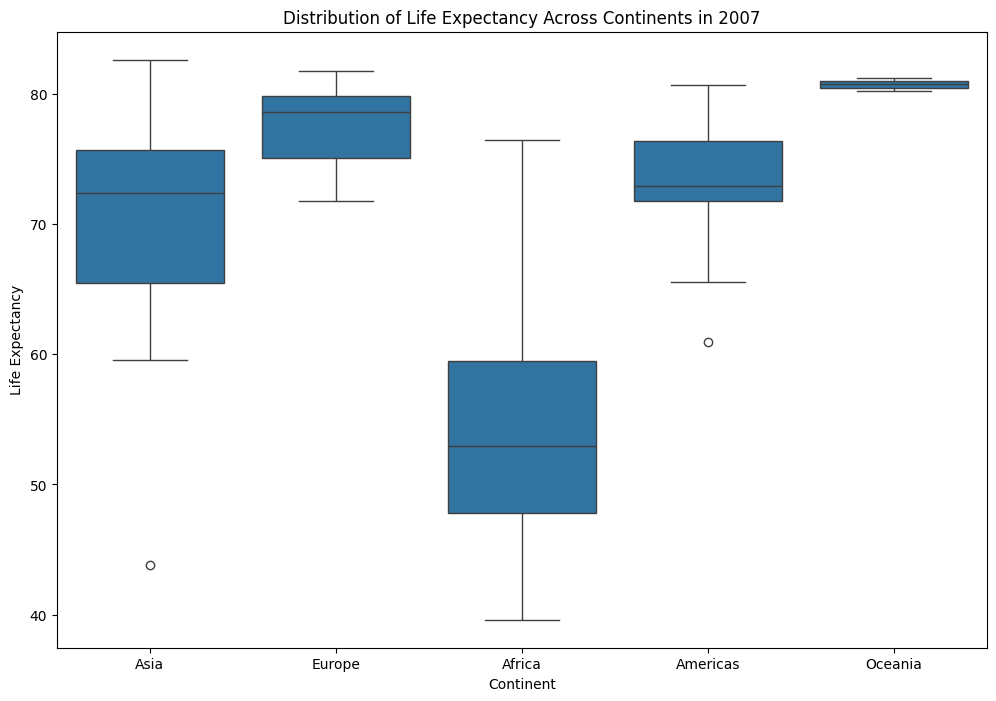
\includegraphics[width=0.5\textwidth]{images/plots/lo1_good_example_life_exp_boxplot.png} 
    \caption{Box plots of the Distribution of Life Expectancy Across Continents in 2007}
    \label{fig:boxplot_good}
\end{figure}

\subsection{Bubble Charts}

Bubble charts are an extension of the scatter plot (Figure \ref{fig:bubble_chart_good}). They allow comparison and portrayal of data points in three dimensions: $x$-coordinate, $y$-coordinate, and size of the bubble. While they are useful for evaluating complex relationships, the size variable can sometimes be misinterpreted. This is because humans are generally less adept at accurately comparing the size of 2D areas than they are at comparing lengths or heights \cite{clevelandGraphicalPerceptionTheory1984}.

\begin{figure}[h]
    \centering
    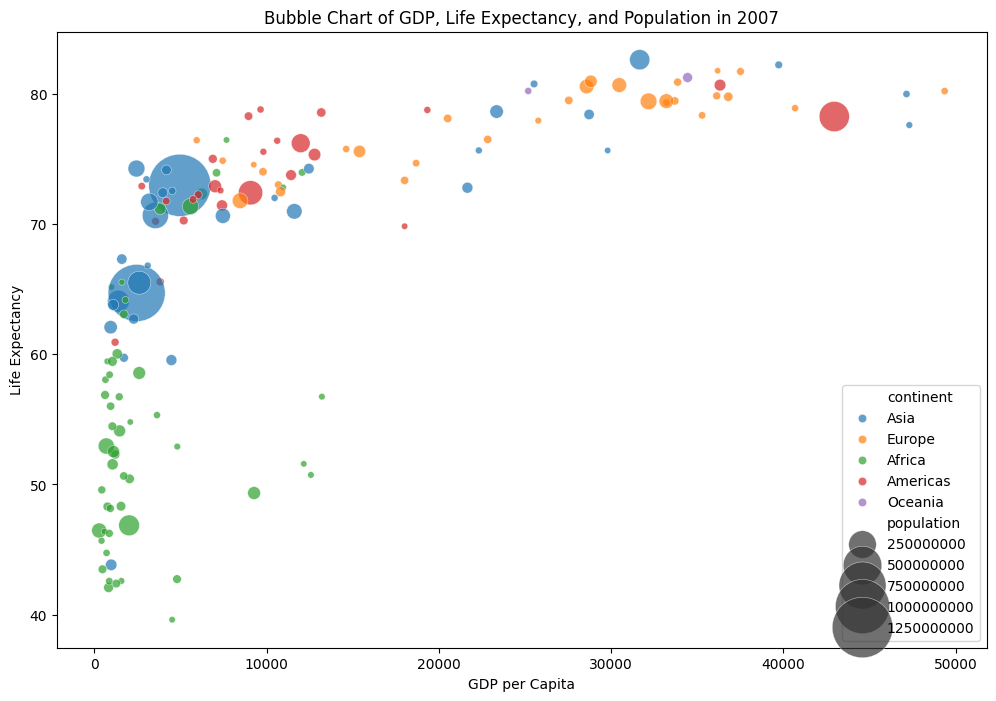
\includegraphics[width=0.5\textwidth]{images/plots/lo1_good_example_bubble_chart.png} 
    \caption{Bubble Chart of GDP, Life Expectancy, and Population in 2007}
    \label{fig:bubble_chart_good}
\end{figure}